\documentclass{journal}

\title{Tic-Tac-Toe by Reinforcement}
\author{Nathaniel Beckemeyer}

% Some packages that I use in every document
\usepackage{comment}
\usepackage{microtype}
\usepackage{booktabs}
\usepackage[utf8]{inputenc}
\usepackage{hyperref}
\usepackage{lmodern}
\usepackage[obeyDraft]{todonotes}

% This document
\usepackage{amsmath}
\usepackage{graphicx}
\graphicspath{{Figures/}}


\begin{document}
\maketitle{}

\section{Introduction}
This project used reinforcment learning to play Tic-Tac-Toe, and specifically
the Sarsa and Q-Learning algorithms, and their respective $\lambda{}$ versions.
I used Sam Beckmann's modified framework for this project, rather than the
one distributed to us.

In this report, the probability of an intermediate reward being given after an
agent makes a move is broken down into four psssibilities according to
Table~\ref{tab:breakdown}. Note that intermediate rewards are always provided
at the end of games.

\begin{table}[h]
\centering{}
\begin{tabular}{lcc}
    & \multicolumn{2}{c}{Probability} \\ \cline{2-3}
    Agent Type & (a) & (b) \\ \toprule
    Deterministic & 1 & 0 \\
    Nondeterministic & 0.75 & 0.50 \\
\end{tabular}
\caption{Description of behaviors}\label{tab:breakdown}
\end{table}

The section that follows is highlights and a brief summary of the results of the
tests that were run and a short discussion. Appendix~\ref{app:optimal} contains
more detailed figures of the runs of the RL players against the optimal players.
See Appendix~\ref{app:rl} for the reinforcement learning agents playing
themselves.

\section{Results \& Discussion}
The results visualized in this report use a 'win percentage' metric; this
percentage is a periodic average; every 50 games the summary data for the
percentages were calculated.

Overall Q-Learning and Sarsa perform similarly---I could notice no substantial
differences in their performances.

The Q-Learning agent learning to defeat the naive agent (in this case, a random
agent) can be seen in Figure~\ref{fig:QLVNaive}. Similarly, the performance
of the Sarsa agent vs the naive agent can be seen in
Figure~\ref{fig:SarsaVNaive}.
\begin{figure}[h]
	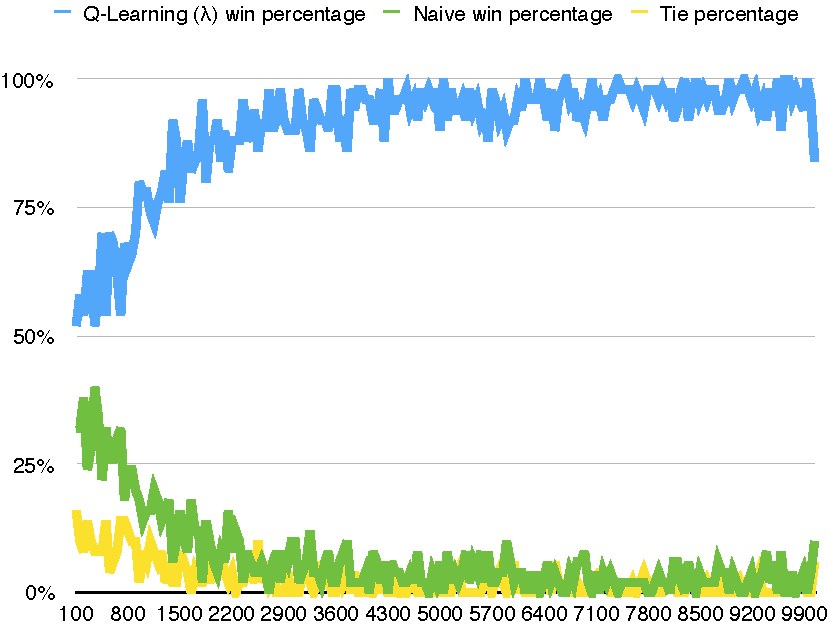
\includegraphics[width=0.8\textwidth]{QLVNaive.pdf}
	\caption{QLearning vs the naive player}\label{fig:QLVNaive}
\end{figure}
\begin{figure}[h]
	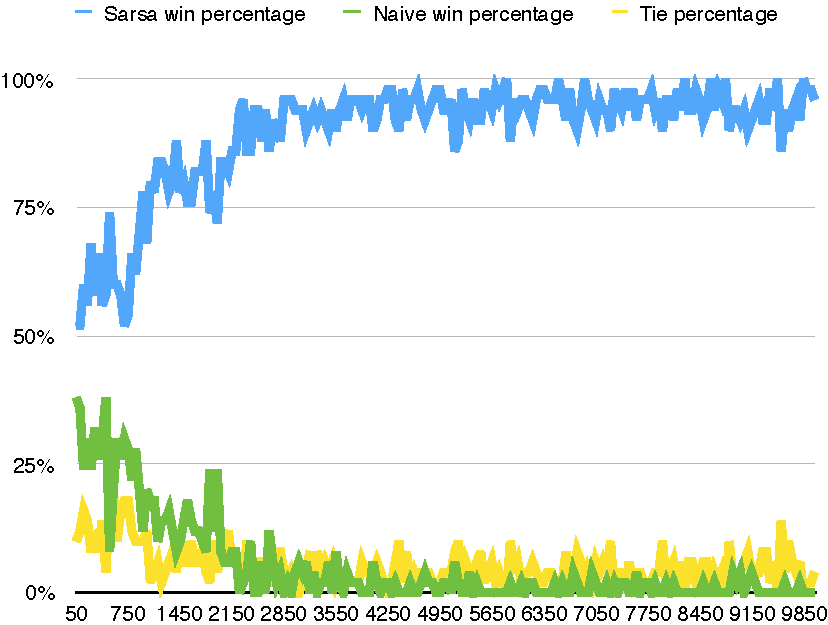
\includegraphics[width=0.8\textwidth]{SarsaVNaive.pdf}
	\caption{Sarsa vs the naive player}\label{fig:SarsaVNaive}
\end{figure}


The most startling result was that both of the $\lambda{}$ players were
outperformed by their non-$\lambda{}$ counterparts! I'm not sure exactly why
this happened, but fortunately the $\lambda{}$ versions do learn to tie the
optimal player. Except for one; interestingly, the Sarsa ($\lambda{}$) player
actually loses to the non-deterministic minimax player with intermediate
rewards. I suspect that the reason for this loss is that Sarsa does not deal
well with the intermediate rewards (which can be incorrect, as they are
based on a minimax and do not distinguish between multiple best moves), hence
why Sarsa generally performs better in the (b) conditions.

Doing this task taught me about the subtle difference and immense similarity
between Sarsa and Q-learning. It also taught me just how quickly RL agents
can learn in small state spaces---the speed difference between my agents and
minimax made me wonder at what point it makes sense to use an RL learner rather
than just a hardcoded solution.


\clearpage{}
\appendix
\section{Optimal player results}\label{app:optimal}
\begin{figure}[h]
	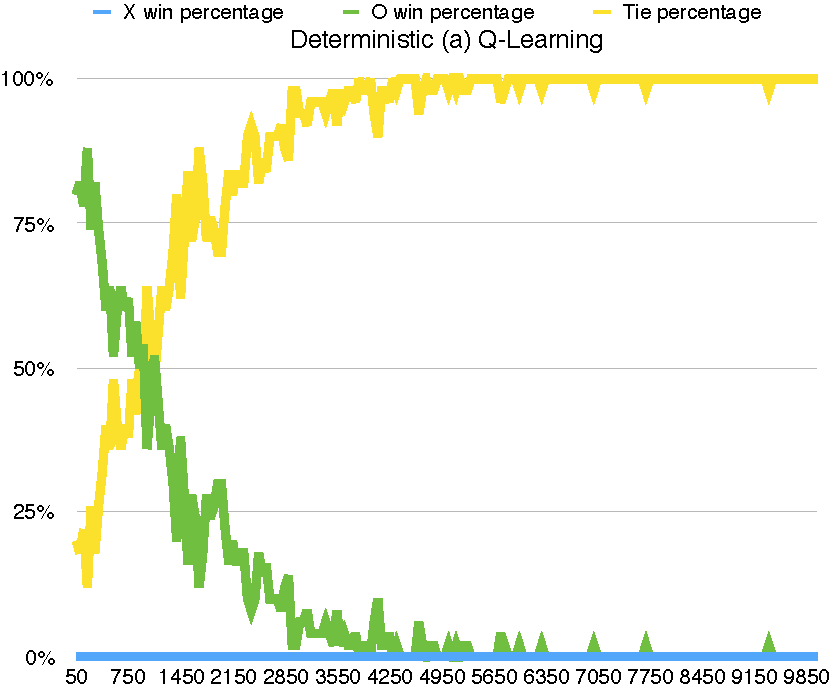
\includegraphics[width=0.8\textwidth]{QLearningD(a).pdf}
	\caption{QLearning with deterministic behavior (a)}\label{fig:QDA}
\end{figure}
\begin{figure}[h]
	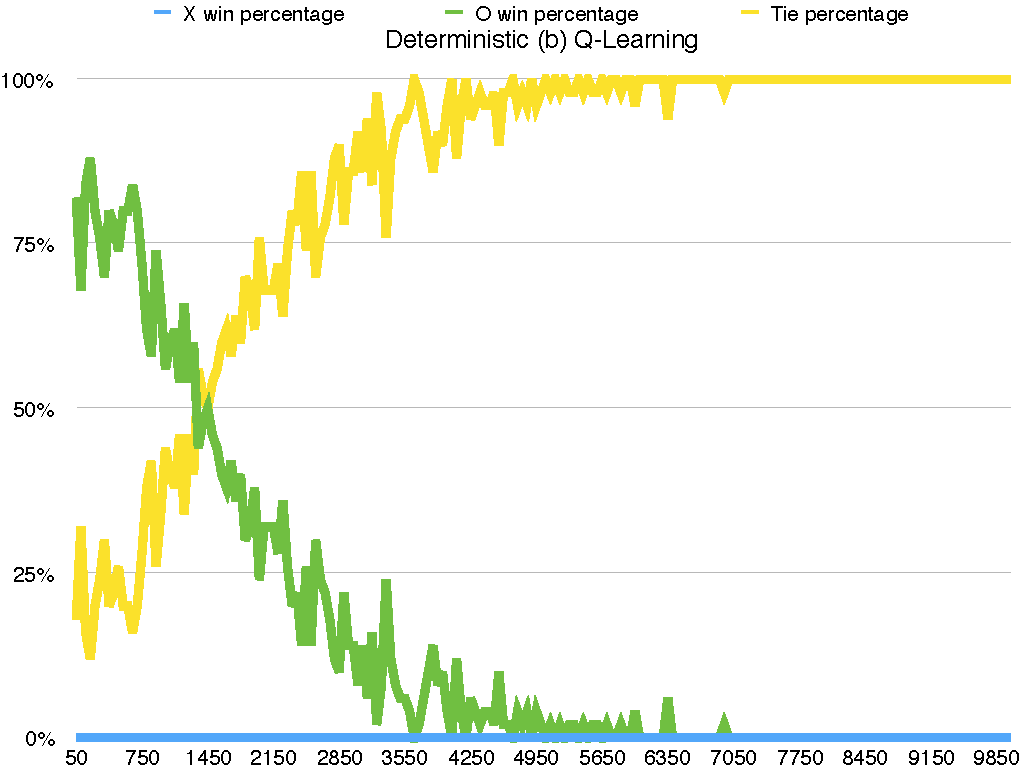
\includegraphics[width=0.8\textwidth]{QLearningD(b).pdf}
	\caption{QLearning with deterministic behavior (b)}\label{fig:QDB}
\end{figure}
\begin{figure}[h]
	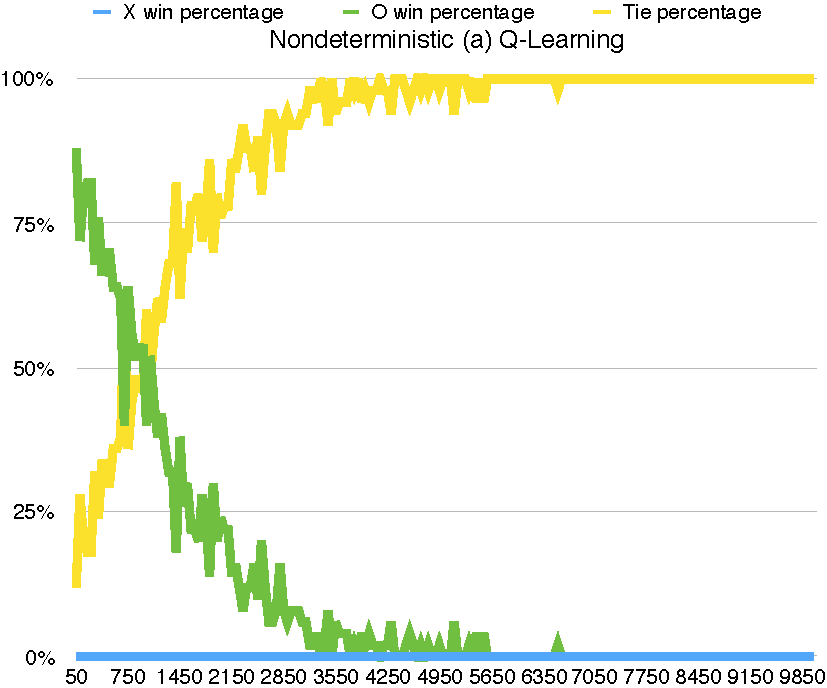
\includegraphics[width=0.8\textwidth]{QLearningN(a).pdf}
	\caption{QLearning with nondeterministic behavior (a)}\label{fig:QNA}
\end{figure}
\begin{figure}[h]
	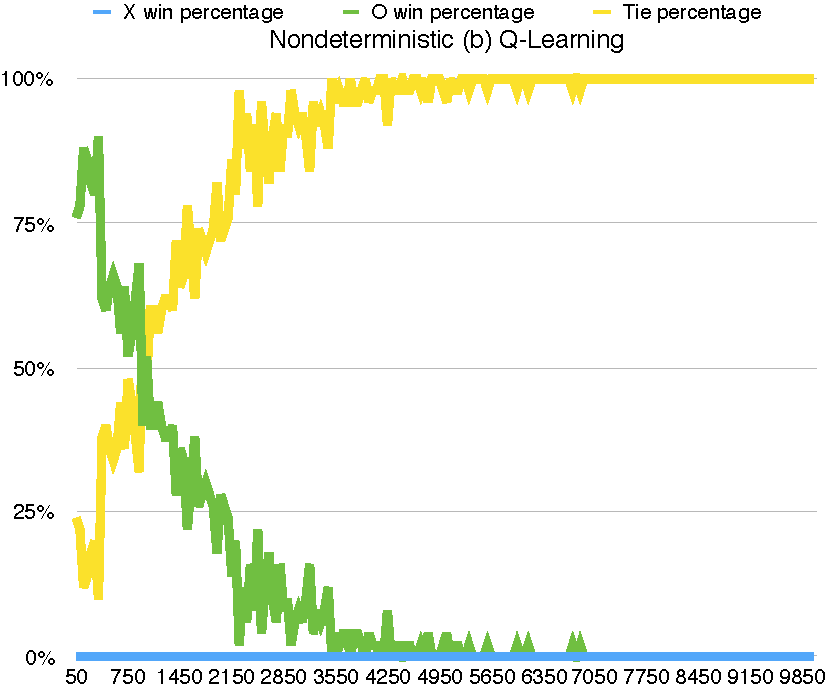
\includegraphics[width=0.8\textwidth]{QLearningN(b).pdf}
	\caption{QLearning with nondeterministic behavior (b)}\label{fig:QNB}
\end{figure}
\begin{figure}[h]
	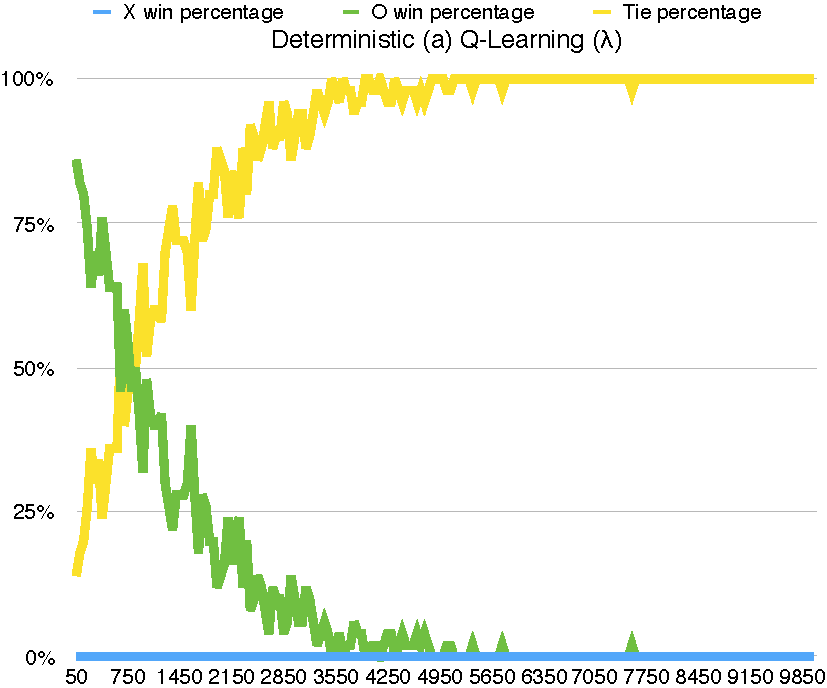
\includegraphics[width=0.8\textwidth]{QLearningLD(a).pdf}
	\caption{QLearning ($\lambda{}$) with deterministic behavior (a)}\label{fig:QLDA}
\end{figure}
\begin{figure}[h]
	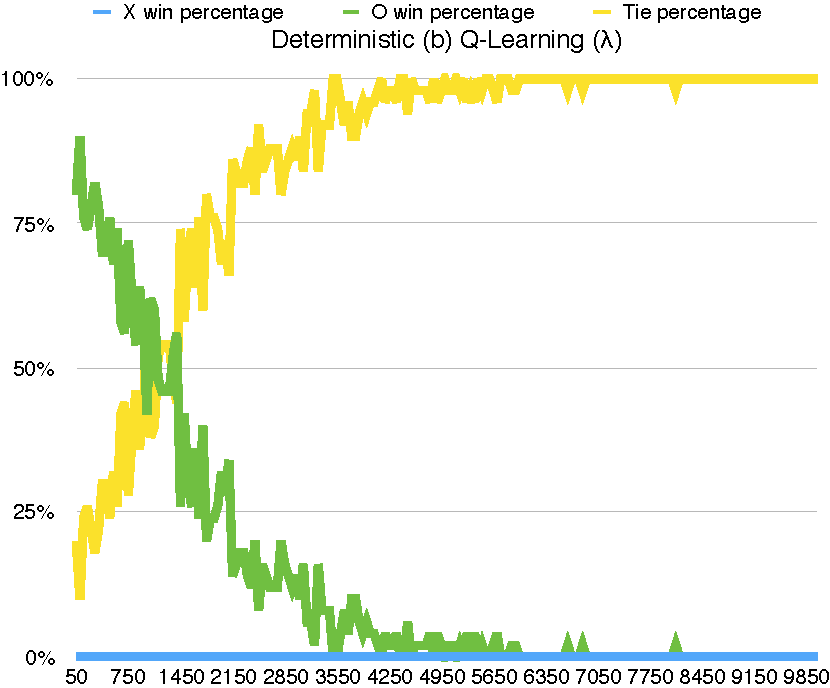
\includegraphics[width=0.8\textwidth]{QLearningLD(b).pdf}
	\caption{QLearning ($\lambda{}$) with deterministic behavior (b)}\label{fig:QLDB}
\end{figure}
\begin{figure}[h]
	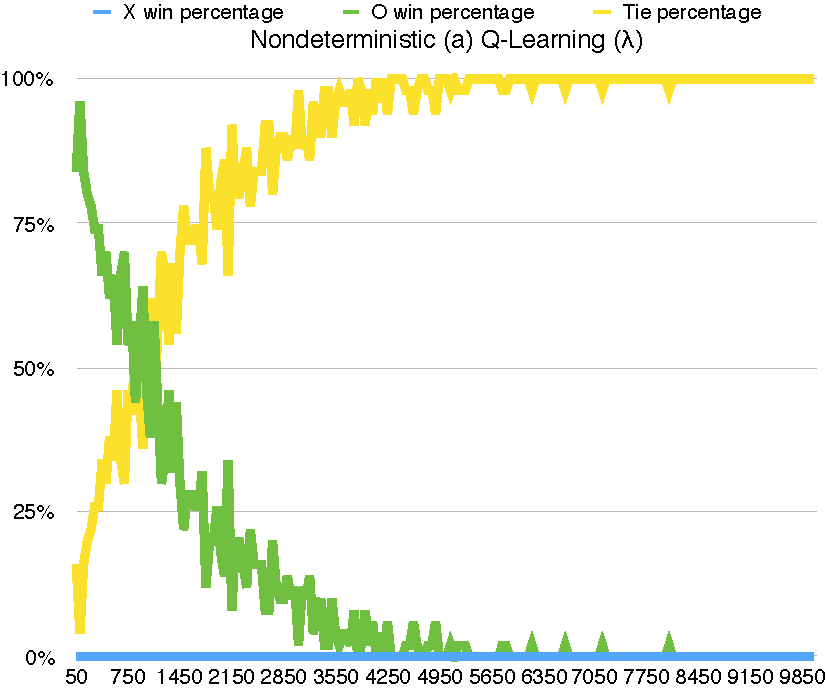
\includegraphics[width=0.8\textwidth]{QLearningLN(a).pdf}
	\caption{QLearning ($\lambda{}$) with nondeterministic behavior (a)}\label{fig:QLNA}
\end{figure}
\begin{figure}[h]
	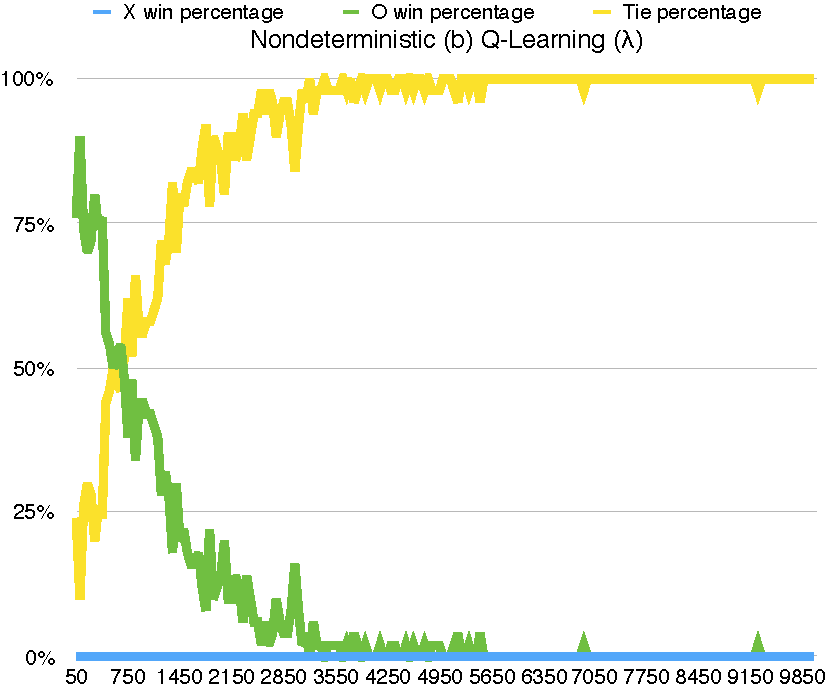
\includegraphics[width=0.8\textwidth]{QLearningLN(b).pdf}
	\caption{QLearning ($\lambda{}$) with nondeterministic behavior (b)}\label{fig:QLNB}
\end{figure}
\begin{figure}[h]
	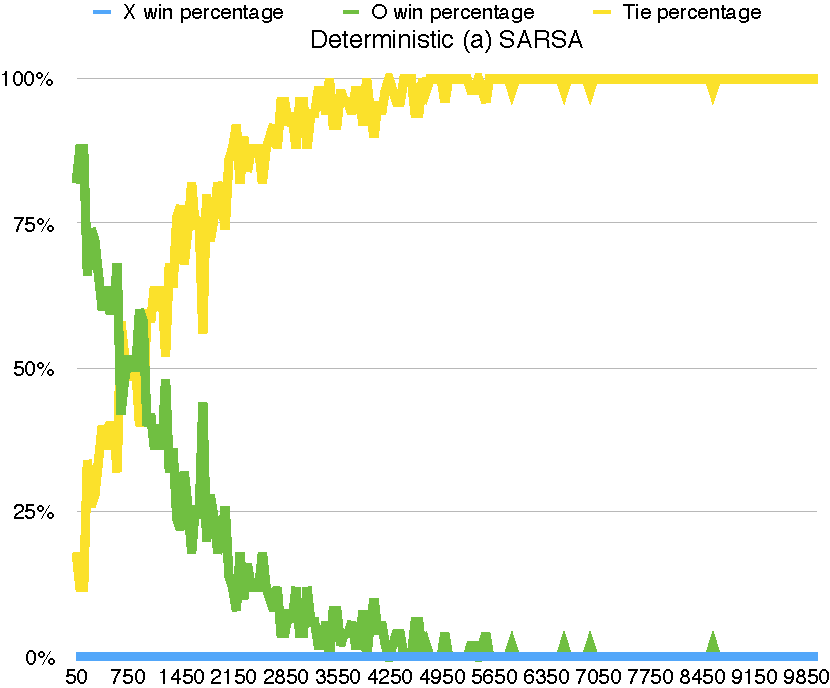
\includegraphics[width=0.8\textwidth]{SarsaD(a).pdf}
	\caption{Sarsa with deterministic behavior (a)}\label{fig:SDA}
\end{figure}
\begin{figure}[h]
	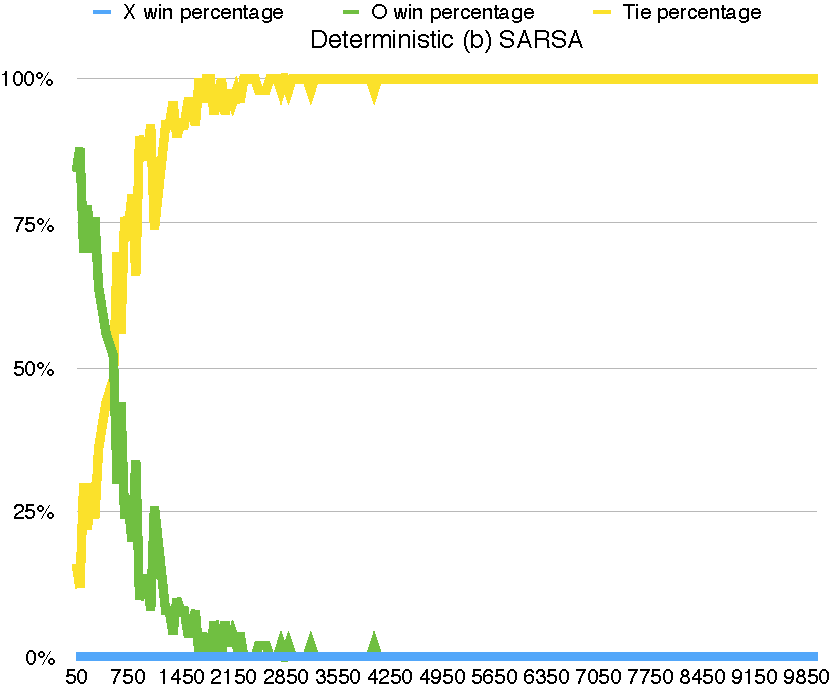
\includegraphics[width=0.8\textwidth]{SarsaD(b).pdf}
	\caption{Sarsa with deterministic behavior (b)}\label{fig:SDB}
\end{figure}
\begin{figure}[h]
	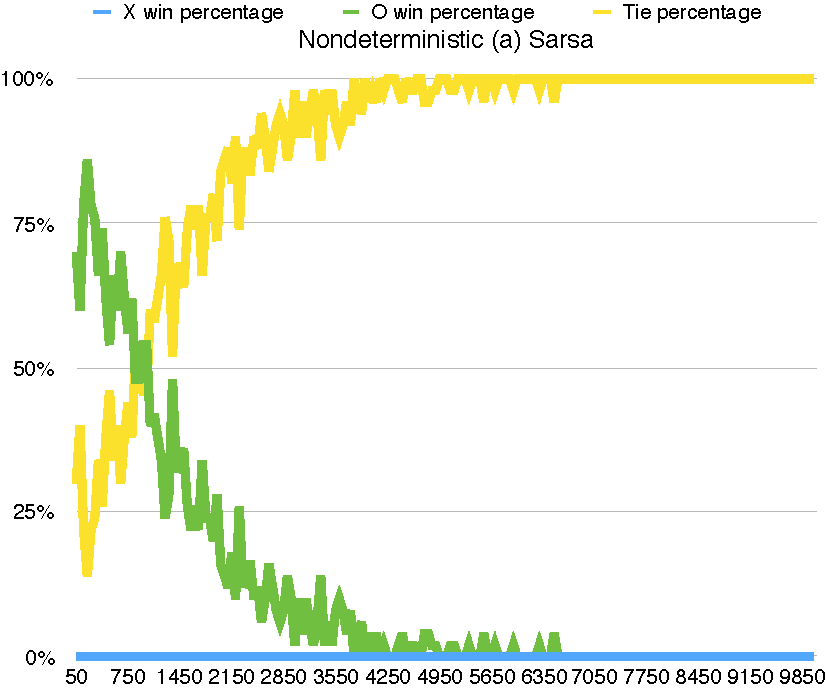
\includegraphics[width=0.8\textwidth]{SarsaN(a).pdf}
	\caption{Sarsa with nondeterministic behavior (a)}\label{fig:SNA}
\end{figure}
\begin{figure}[h]
	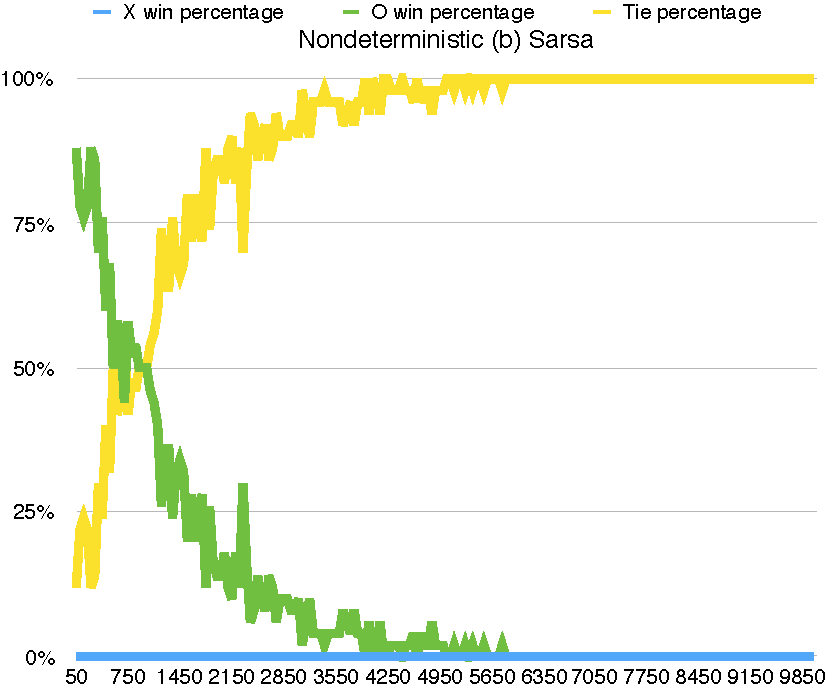
\includegraphics[width=0.8\textwidth]{SarsaN(b).pdf}
	\caption{Sarsa with nondeterministic behavior (b)}\label{fig:SNB}
\end{figure}
\begin{figure}[h]
	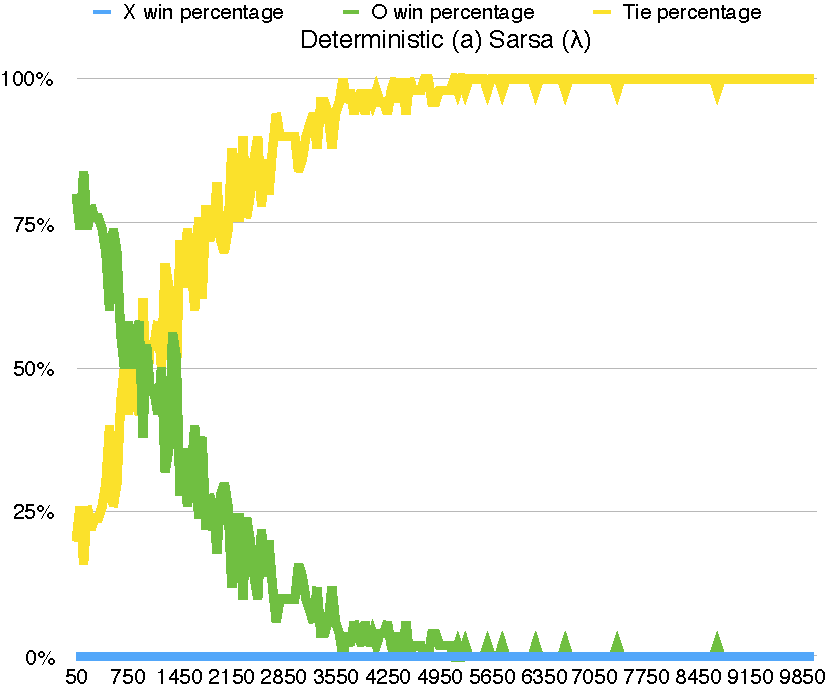
\includegraphics[width=0.8\textwidth]{SarsaLD(a).pdf}
	\caption{Sarsa ($\lambda{}$) with deterministic behavior (a)}\label{fig:SLDA}
\end{figure}
\begin{figure}[h]
	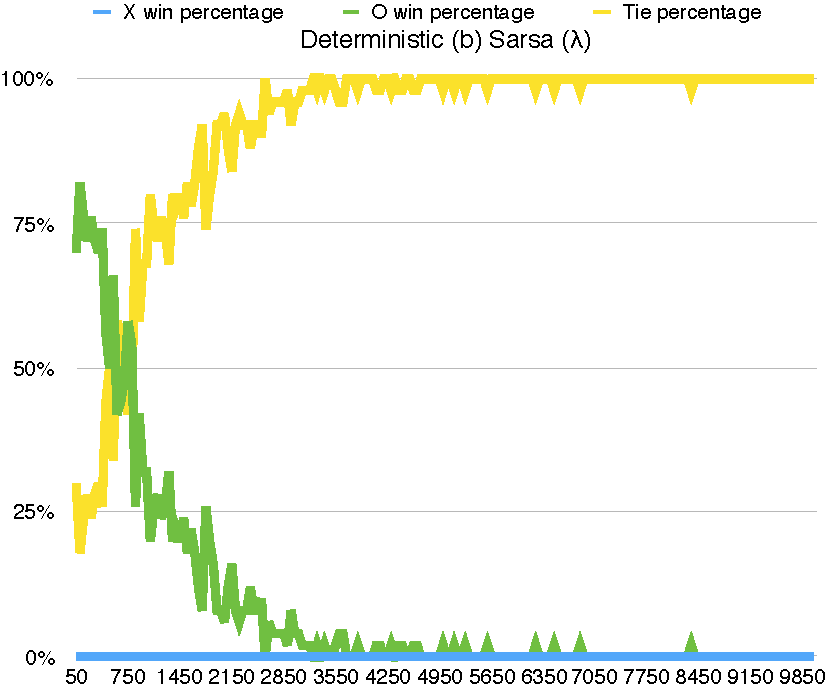
\includegraphics[width=0.8\textwidth]{SarsaLD(b).pdf}
	\caption{Sarsa ($\lambda{}$) with deterministic behavior (b)}\label{fig:SLDB}
\end{figure}
\begin{figure}[h]
	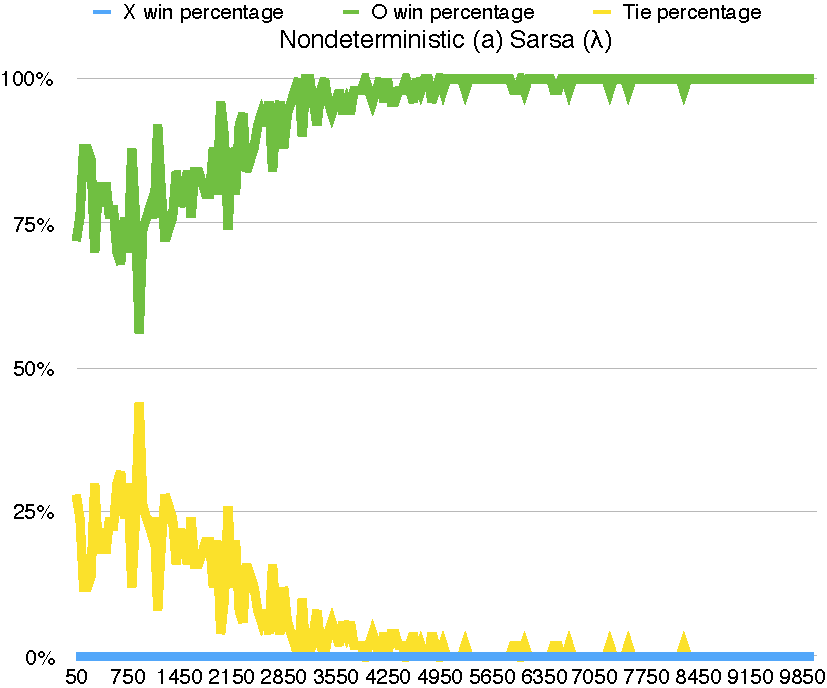
\includegraphics[width=0.8\textwidth]{SarsaLN(a).pdf}
	\caption{Sarsa ($\lambda{}$) with nondeterministic behavior (a)}\label{fig:SLNA}
\end{figure}
\begin{figure}[h]
	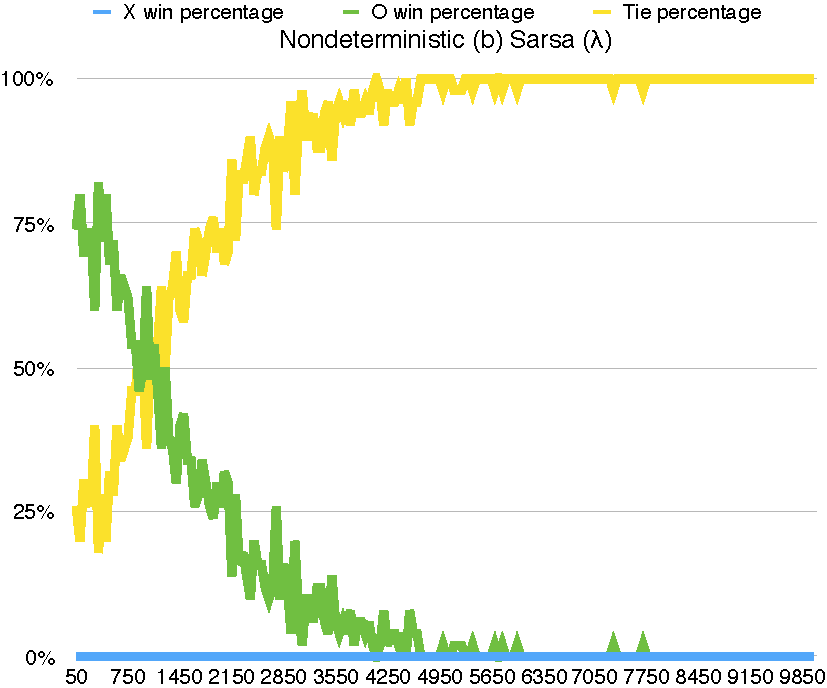
\includegraphics[width=0.8\textwidth]{SarsaLN(b).pdf}
	\caption{Sarsa ($\lambda{}$) with nondeterministic behavior (b)}\label{fig:SLNB}
\end{figure}


\clearpage{}
\section{RL against itself}\label{app:rl}
\begin{figure}[h]
	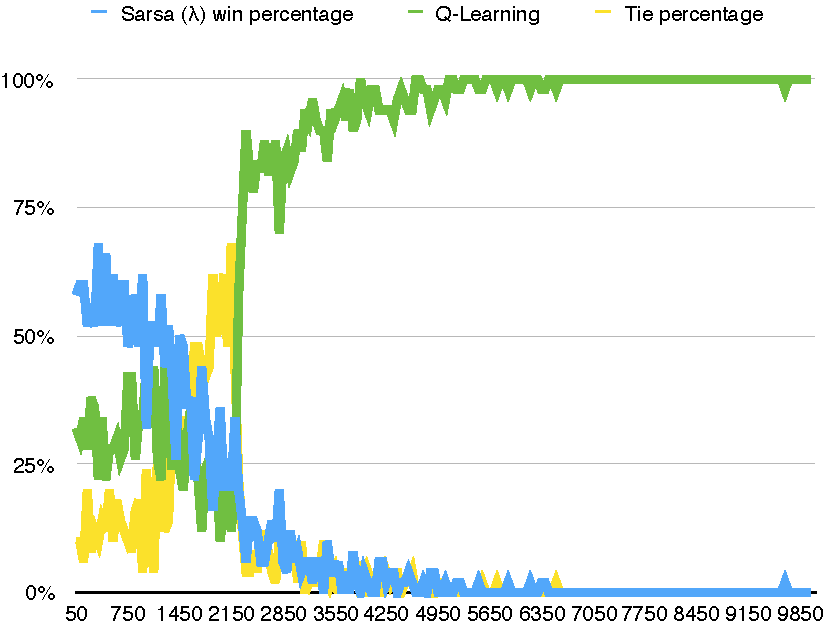
\includegraphics[width=0.8\textwidth]{SLVQ.pdf}
	\caption{Sarsa ($\lambda{}$) against a Q-Learner}
\end{figure}
\begin{figure}[h]
	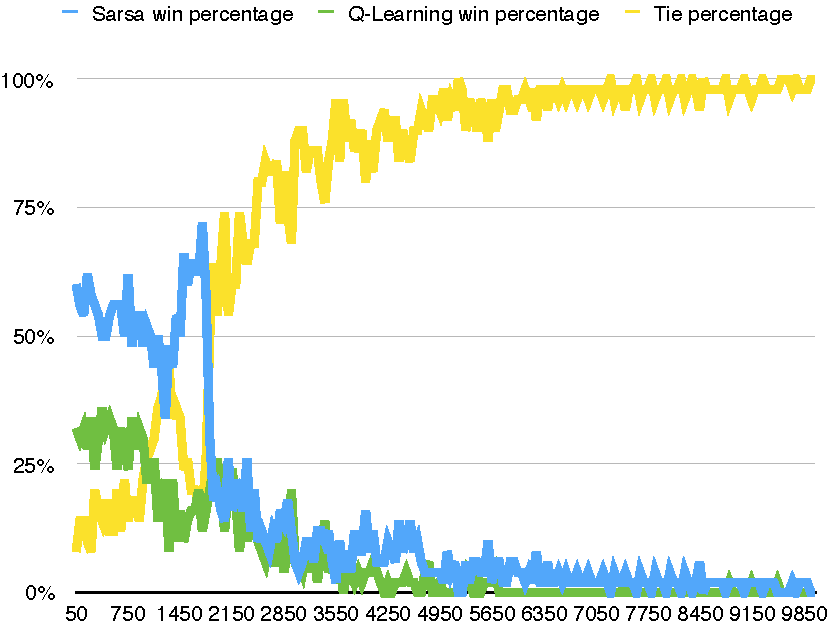
\includegraphics[width=0.8\textwidth]{SVQ.pdf}
	\caption{Sarsa against a Q-Learner}
\end{figure}
\begin{figure}[h]
	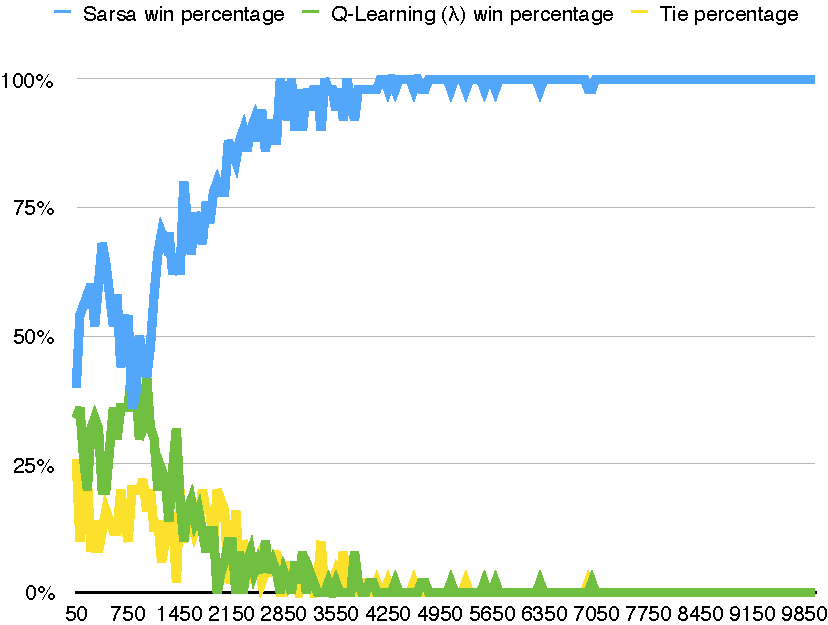
\includegraphics[width=0.8\textwidth]{SVQL.pdf}
	\caption{Sarsa against a Q ($\lambda{}$)-Learner}
\end{figure}
\begin{figure}[h]
	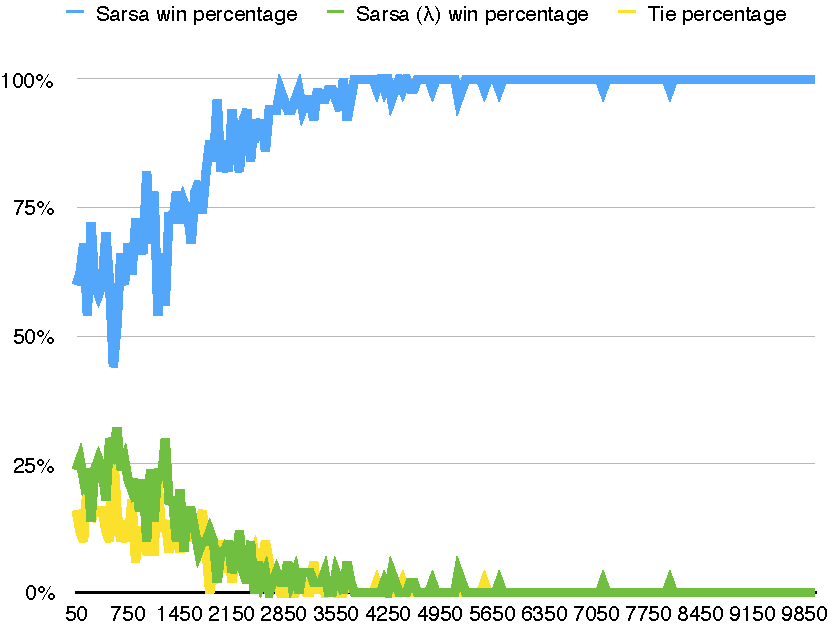
\includegraphics[width=0.8\textwidth]{SVSL.pdf}
	\caption{Sarsa against a Sarsa ($\lambda{}$)-Learner}
\end{figure}
\begin{figure}[h]
	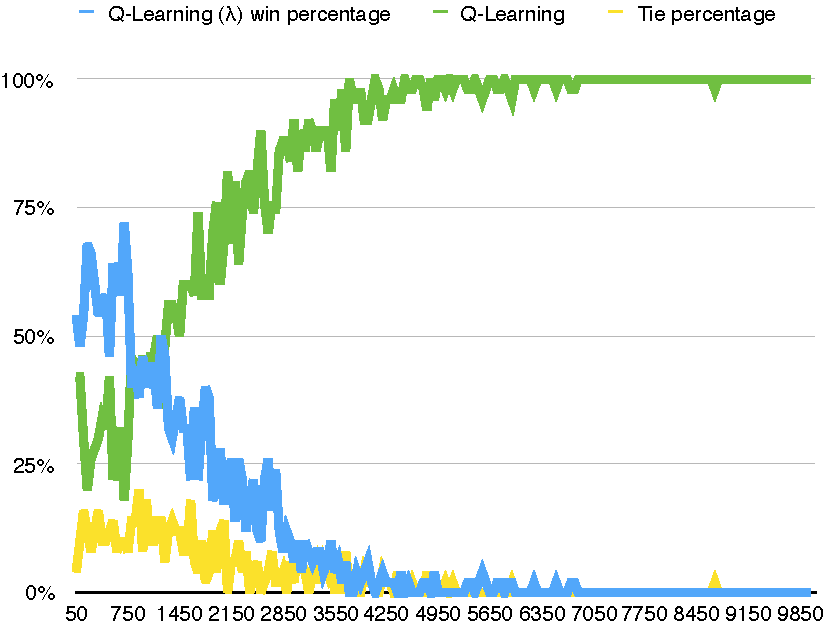
\includegraphics[width=0.8\textwidth]{QLVQ.pdf}
	\caption{Q($\lambda{}$) against a Q-Learner}
\end{figure}
\begin{figure}[h]
	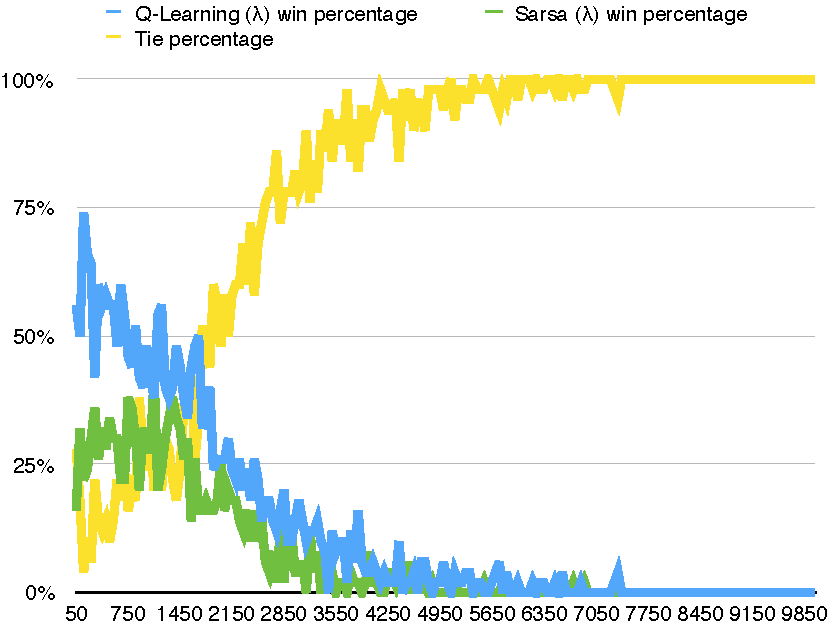
\includegraphics[width=0.8\textwidth]{QLVSL.pdf}
	\caption{Q($\lambda{}$) against a Sarsa ($\lambda{}$)-Learner}
\end{figure}



\end{document}
